\documentclass[a4paper, 12pt]{article}
\usepackage{style}

%colori per tablle tabu
\definecolor{tableHeader}{RGB}{254, 61, 0}
\definecolor{tableLineOne}{RGB}{245, 245, 245}
\definecolor{tableLineTwo}{RGB}{254, 204, 188}
%define header tabelle tabu
\newcommand{\tableHeaderStyle}{
    \rowfont[c]{\leavevmode\color{white}\bfseries}
    \rowcolor{tableHeader}
}

\title{PianoDiQualifica}
\author{Cyber13}
\date{March 2019}

\begin{document}
	\begin{titlepage}
		\centering Università degli Studi di Padova
		\line(1,0){350}\\
		\vspace{1.2cm}
		\logo
		\vspace{1.0cm}
		\centering{\bfseries\LARGE PIANO DI QUALIFICA \\}
		\vspace{0.5cm}
		\centering{\slshape\large Gruppo Cyber13 - Progetto P2PCS\\}
		\vspace{0.5cm}
		\centering{\bfseries Informazioni sul documento \\}
		\line(1,0){240}\\
		% compilare i campi per ogni documento
		\begin{tabular}{r|l}
			{\textbf{Versione}} 			& 1.0.0\\
			{\textbf{Data Redazione}} 	& 04/04/2019\\	% aggiornare la data
			{\textbf{Responsabili}} 	& Elena Pontecchiani \\ & Andrea Casagrande \\	% aggiornare la data
			{\textbf{Redazione}} 		& Daniel Mirel Bira \\ & Andrea Casagrande \\ & Ilaria Rizzo\\ & Matteo Squeri\\
			{\textbf{Verifica}} 		 & Fabio Garavello \\ & Ilaria Rizzo\\
			{\textbf{Approvazione}} 		& Andrea Casagrande\\
			{\textbf{Uso}} 				& Esterno\\
			{\textbf{Destinatari}} & GaiaGo\\	& Cyber13\\ & Prof. Tullio Vardanega\\ & Prof. Riccardo Cardin\\
			{\textbf{Mail di contatto}} 	& swe.cyber13@gmail.com\\
		\end{tabular}\\
	\end{titlepage}

    \newpage
		\subfile{DiarioModifiche.tex}
	\newpage
		\tableofcontents
    \newpage
	     \listoffigures
	\newpage
        \section{Introduzione}
        \subsection{Scopo del documento}
Il presente documento ha il compito di descrivere le motivazioni che hanno portato i componenti del team Cyber13 alla scelta dello svolgimento del \citgl{capitolato} C5. La scelta è stata effettuata tenendo conto dei seguenti fattori:
    \begin{itemize}
        \item Le proposte dei vari progetti e quello che richiedono di implementare.
        \item Le tecnologie che i progetti richiedono per il loro sviluppo. Considerando che il gruppo si colloca nel \citgl{secondo lotto} e che la maggioranza degli studenti ha esami arretrati, si è preferito avvantaggiare progetti che proponessero tecnologie almeno in parte conosciute dai componenti.
        \item I progetti ancora disponibili. I progetti non più a disposizione sono stati scartati.
    \end{itemize}
		            
\subsection{Glossario}
Onde evitare ambiguità o incomprensioni di natura lessicale, si allega il \G.
All'interno del documento saranno presenti parole di ambito specifico, uso raro che potrebbero creare incomprensioni. Per una maggiore leggibilità tali parole sono riconoscibili all'interno dei vari documenti in quanto scritte in corsivo e con un 'g' a pedice tra barre orizzontali (per esempio \citgl{Glossario})
    
\subsection{Riferimenti}
    \subsubsection{Riferimenti normativi}
        \begin{itemize}
            \item \NdP
        \end{itemize}
    
    \subsubsection{Riferimenti informativi}
        \begin{itemize}
            \item Capitolato C1:\\ \url{https://www.math.unipd.it/~tullio/IS-1/2018/Progetto/C1.pdf}
            \item Capitolato C2:\\ \url{https://www.math.unipd.it/~tullio/IS-1/2018/Progetto/C2.pdf}
            \item Capitolato C3:\\ \url{https://www.math.unipd.it/~tullio/IS-1/2018/Progetto/C3.pdf}
            \item Capitolato C4:\\ \url{https://www.math.unipd.it/~tullio/IS-1/2018/Progetto/C4.pdf}
            \item Capitolato C5:\\ \url{https://www.math.unipd.it/~tullio/IS-1/2018/Progetto/C5.pdf}
            \item Capitolato C6:\\ \url{https://www.math.unipd.it/~tullio/IS-1/2018/Progetto/C6.pdf}
        \end{itemize}
   
    \newpage
        \section{Qualità di processo}
        La qualità finale di un prodotto è determinata in maniera decisiva dalla qualità dei processi che portano alla produzione dello stesso, per questo motivo il team ha deciso di adottare lo standard ISO/IEC 15504 conosciuto anche come \citgl{SPICE} il quale definisce un modello di valutazione dello stadio di maturità di un processo. SPICE prevede sei livelli di maturità per un dato processo e per ognuno di essi definisce anche degli attributi di processo che permettono di determinare con maggior precisione se un livello di maturità viene raggiunto o meno dal processo in questione. In questo documento verranno citate solo le voci ritenute rilevanti in relazione al contesto.
\\\\
\textbf{Level 0 - Incomplete process:} il processo non è implementato o non raggiunge gli obiettivi prefissati, gli output del processo sono pochi o inesistenti. Gli attributi di tale processo sono:
\begin{itemize}
    \item non sono previsti attributi di processo per questo livello.
\end{itemize}
\\\\
\textbf{Level 1 - Performed process:} il processo viene attuato e raggiunge gli obiettivi prefissati, tuttavia non viene scrupolosamente controllato. Gli attributi di tale processo sono: 
\begin{itemize}
    \item \textbf{P.A. 1.1 - Performed process:} capacità di raggiungere i propri obiettivi e produrre output identificabili.
\end{itemize}
\\\\
\textbf{Level 2 - Managed process:} il processo viene attuato, controllato, tracciato e gli output prodotti raggiungono standard prefissati. Gli attributi di tale processo sono:
\begin{itemize}
    \item \textbf{P.A. 2.1 - Performance management:} capacità di produrre output che raggiungono gli obiettivi prefissati;
    \item \textbf{P.A. 2.2 - Work product management:} capacità di produrre output controllato e tracciato.
\end{itemize}
\\\\
\textbf{Level 3 - Established process:} il processo viene attuato e controllato seguendo i principi dell'ingegneria del software. Gli attributi di tale processo sono:
\begin{itemize}
    \item \textbf{P.A. 3.1 - Process definition:} capacità di produrre output che si attengano agli standard dell'ingegneria del software;
    \item \textbf{P.A. 3.2 - Process resource:} capacità di produrre output efficacemente utilizzando una quantità di risorse ragionevole.
\end{itemize}
\\\\
\textbf{Level 4 - Predictable process:} il processo viene attuato con vincoli determinati a raggiungere gli obbiettivi previsti. Il processo risulta essere ben collaudato nella pratica. Gli attributi di tale processo sono:
\begin{itemize}
    \item \textbf{P.A 4.1 - Process measurement:} capacità di utilizzare le misure ottenute durante l'esecuzione del processo per verificare in futuro il raggiungimento degli obiettivi prefissati;
    \item \textbf{P.A. 4.2 Process control:} capacità di modificare l'esecuzione del processo in seguito ai dati raccolti
\end{itemize}
\\\\
\textbf{Level 5 - Optimizing process:} il processo ha una certa consistenza nel raggiungere i propri obiettivi, viene ottimizzato per adempiere al meglio agli obiettivi correnti e futuri. gli attributi di tale processo sono:
\begin{itemize}
    \item \textbf{P.A. 5.1 - Process change:} capacità di tracciare tutti i cambiamenti del processo, siano essi strutturati o di esecuzione;
    \item \textbf{P.A. 5.2 - Continuous improvement:} capacità di implementare le modifiche applicate.
\end{itemize}
\\
Per tutti gli attributi di processo, SPICE fornisce un metodo di valutazione per misurare il loro raggiungimento:
\begin{itemize}
    \item \textbf{N:} non posseduto (0\% - 15\%);
    \item \textbf{P:} parzialmente posseduto (16\% - 50\%);
    \item \textbf{L:} largamente posseduto (51\% - 85\%);
    \item \textbf{F:} totalmente posseduto (86\% - 100\%).
\end{itemize}
\\
Tali valori possono essere utilizzati nel ciclo \citgl{PDCA} il cui scopo è quello di controllare la qualità di un processo durante tutto il suo ciclo di vita e permettere il miglioramento in efficacia ed efficienza dello stesso. Le fasi descritte da PDCA sono le seguenti:
\begin{itemize}
    \item \textbf{Plan:} fase di pianificazione dove si decidono e si individuano gli obiettivi di qualità e i risultati desiderati;
    \item \textbf{Do:} fase in cui si mette in atto il piano stabilito nella fase precedente;
    \item \textbf{Check:} fase di vendita in cui si confrontano i dati in output della fase Do con i risultati previsti in fase Plan;
    \item \textbf{Act:} fase in cui si individuano le cause delle eventuali discordanze riscontrate in fase di Check e si determinano le azioni da intraprendere per risolvere tali discordanze e migliorare il processo aumentandone cosi la qualità.
\end{itemize}
\\\\
Il gruppo ha inoltre individuato nello standard ISO/IEC 12207 alcuni processi il cui scopo è quello di garantire la qualità del prodotto finale. In questo documento verranno citate solo le voci ritenute rilevanti in relazione al contesto.

\subsection{PROC[0001] - Project assessment and Control Process}
Lo scopo di questo processo è quello di determinare lo stato del lavoro svolto ed assicurare che il tutto si stia svolgendo secondo i piani ed entro i limiti di risorse e tempo prestabiliti.
\subsubsection{Obiettivi}
\begin{itemize}
    \item Ogni membro del gruppo svolgerà il \citgl{task} assegnatogli nei tempi previsti;
    \item Le risorse impiegate per una fase non dovranno superare i limiti prestabiliti.
\end{itemize}

\subsubsection{Strategie} 
Il \citgl{Project Manager} deve monitorare lo svolgimento del processo in modo da rilevare il prima possibile eventuali ritardi nello svolgimento dei task e/o un utilizzo delle risorse superiore ai limiti prestabiliti. In caso di rilevamento di tale eccedenza, il gruppo dovrà assolutamente risolvere il problema entro la data prevista per la consegna finale del prodotto.

\subsubsection{Metriche}
\paragraph{M[PROC][0001] - Schedule Variance} 
\begin{itemize}
    \item \textbf{Range di accettazione}: >= 0
    \item \textbf{Range ottimale}: >= 0
\end{itemize}

\paragraph{M[PROC][0002] - Budget Variance} 
\begin{itemize}
    \item \textbf{Range di accettazione}: >= 0
    \item \textbf{Range ottimale}: >= 0
\end{itemize}

\subsection{PROC[0002] - Risk Management Process}
Lo scopo di questo processo è quello di individuare, analizzare e monitorare i rischi durante l'intera durata del progetto.

\subsubsection{Obiettivi}
\begin{itemize}
    \item Il gruppo individuerà i rischi nella prima fase del progetto e ne terrà traccia fino a quando il rischio non sarà più una possibile evenienza;
    \item L'individuazione del rischi verrà svolta ad ogni fase in modo da identificare nuovi possibili rischi introdotti dalle attività svolte nella fase precedente.
\end{itemize}

\subsubsection{Strategie}
Il gruppo dovrà tenere sempre sotto stretta osservazione tutti i rischi in modo da poter mitigare al meglio l'eventuale manifestazione.

\subsubsection{Metriche}
\paragraph{M[PROC][0003] - Rischi non individuati}
\begin{itemize}
    \item \textbf{Range di accettazione}: 0 - 4
    \item \textbf{Range ottimale:} 0
\end{itemize}

\subsection{PROC[0003] - Software Detailed Design Process}
Lo scopo di questo processo è fornire una progettazione di dettaglio del prodotto che andrà ad implementare i requisiti individuati.

\subsubsection{Obiettivi}
\begin{itemize}
    \item Il grado di dettaglio della progettazione deve fornire sufficiente informazione per procedere alla codifica e testing di un'unità senza bisogno di ulteriori informazioni.
\end{itemize}

\subsubsection{Strategie}
Le componenti individuate durante l'analisi verranno suddivise in piccole unità codificabili e testabili facilmente.

\subsubsection{Metriche}

    \paragraph{M[PROC][0004]: Numero campi dati per classe}
\begin{itemize}
    \item \textbf{Range di accettazione}: 0-16
    \item \textbf{Range ottimale}: 0-10
\end{itemize}

\paragraph{M[PROC][0005] - Metodi per classe}
\begin{itemize}
    \item \textbf{Range di accettazione}: 1-10
    \item \textbf{Range ottimale}: 1-7
\end{itemize}

\paragraph{M[PROC][0006] - Parametri per metodo} 
\begin{itemize}
    \item \textbf{Range di accettazione}: 0-8
    \item \textbf{Range ottimale}: 0-5
\end{itemize}


\paragraph{M[PROC][0007]: Grado di instabilità}
\begin{itemize}
    \item \textbf{Range di accettazione}: 0-0.8
    \item \textbf{Range ottimale}: 0.3-0.7
    \end{itemize}
    
\subsection{PROC[0004] - Software Construction Process}
Lo scopo di questo processo è definire le attività principali volte alla produzione di unità software.

\subsubsection{Obiettivi}
\begin{itemize}
    \item il codice prodotto dovrà risultare di bassa complessità per facilitarne la verifica e la complessità;
    \item sdoppiamenti di flusso verranno ridotti al minimo necessario;
    \item il codice prodotto dovrà risultare facilmente manutenibile.
\end{itemize}

\subsubsection{Strategie}
Il team si impegna a mantenere una complessità bassa nella stesura del codice.

\subsubsection{Metriche}
\paragraph{M[PROC][0008] - Complessità Ciclomatica}
\begin{itemize}
    \item \textbf{Range di accettazione}: 1-15
    \item \textbf{Range ottimale}: 1-10
\end{itemize}

\paragraph{M[PROC][0009] - Linee di codice per linee di comando} 
\begin{itemize}
    \item \textbf{Range di accettazione}: >=25
    \item \textbf{Range ottimale}: >=30
\end{itemize}

\paragraph{M[PROC][0010] - Halstead Difficulty per-function}
\begin{itemize}
    \item \textbf{Range di accettazione}: 0-25
    \item \textbf{Range ottimale:} 0-10
\end{itemize}

\paragraph{M[PROC][0011] - Halstead Volume per-function} 
\begin{itemize}
    \item \textbf{Range di accettazione}: 20-1500
    \item \textbf{Range ottimale:} 20-1000
\end{itemize}

\paragraph{M[PROC][0012] - Halstead Effort per-function} 
Rappresenta il costo necessario a scrivere il codice di una funzione.
\begin{itemize}
    \item \textbf{Range di accettazione}: 0-400
    \item \textbf{Range ottimale:} 0-300
\end{itemize}

\paragraph{M[PROC][0013] - Indice di manutenibilità}
\begin{itemize}
    \item \textbf{Range di accettazione}: 100-171
    \item \textbf{Range ottimale:} 120-171
\end{itemize}

\subsection{PROC[0005] - Test}

\subsubsection{Scopo} 
Lo scopo è di definire una misurazione per l'esecuzione dei test e relativi fallimenti
\paragraph{M[PROC][TM][0001] - Percentuale di codice coperto da test}
\begin{itemize}
    \item \textbf{Range di accettazione}: >=0\%
    \item \textbf{Range ottimale}: 100\%
\end{itemize}

\paragraph{M[PROC][TM][0002] - Percentuale di test passati}
\begin{itemize}
    \item \textbf{Range di accettazione}: 100\%
    \item \textbf{Range ottimale}: 100\%
\end{itemize}

\paragraph{M[PROC][TM][0003] - Percentuale di test non passati}
\begin{itemize}
    \item \textbf{Range di accettazione}: 0\%;
    \item \textbf{Range ottimale}: 0\%.
\end{itemize}


    \newpage
        \section{Qualità di prodotto}
        \subsection{Scopo}
A seguito dello studio dello standard ISO/IEC 9126 il gruppo ha deciso di adottarne alcuni concetti per garantire la qualità del prodotto, esaminata di seguito con obiettivi e metriche corrispondenti.

\subsection{Qualità dei documenti}
I documenti devono essere corretti dal punto di vista ortografico, sintattico, logico, e a livello di leggibilità e comprensibilità.

\subsubsection{Obiettivi: Comprensione}
Il documento deve presentarsi corretto dal punto di vista ortografico e con una leggibilità almeno per persone con licenza media.
\subsubsection{Metriche per documenti}
\paragraph{M[PROD][D][0001]: Indice di \citgl{Gulpease}}
\begin{itemize}
    \item \textbf{Range di accettazione}: 50-100;
    \item \textbf{Range ottimale}: 60-100.
\end{itemize}
\paragraph{M[PROD][D][0002]: Errori ortografici}
\begin{itemize}
    \item \textbf{Range di accettazione}: 100\% corretto;
    \item \textbf{Range ottimale}: 100\% corretto.
\end{itemize}

\subsection{Qualità del software}
\subsubsection{Obiettivi} 
Lo standard ISO/IEC 9126 scelto dal gruppo stabilisce che il modello di qualità sia rappresentato dalle seguenti sei caratteristiche generali, e dalle loro sotto categorie:
\paragraph{Funzionalità}
~\\
Il gruppo si impegna a creare un prodotto software in grado di soddisfare al 100\% i requisiti obbligatori previsti in \AdR  (Accuratezza) fornendo un appropriato insieme di funzionalità (Appropriatezza).
\subparagraph{M[PROD][S][0001]: Copertura requisiti obbligatori}
\begin{itemize}
    \item \textbf{Range di accettazione}: 100\%
    \item \textbf{Range ottimale}: 100\%
\end{itemize}
\subparagraph{M[PROD][S][0002]: Copertura requisiti accettati}
\begin{itemize}
    \item \textbf{Range di accettazione}: 0-100\%
    \item \textbf{Range ottimale}: 100\%
\end{itemize}
\subparagraph{M[PROD][S][0003]: Accuratezza rispetto alle attese}
\begin{itemize}
    \item \textbf{Range di accettazione}: 75-100\%
    \item \textbf{Range ottimale}: 100\%
\end{itemize}

\paragraph{Affidabilità}
~\\
Allo scopo di creare un prodotto software affidabile verranno presi in considerazione i seguenti parametri. Maturità, intesa come capacità dell'applicativo di evitare più possibile errori e malfunzionamenti. Tolleranza agli errori, intesa come capacità invece di gestire tali errori e malfunzionamenti qualora si verificassero.

\subparagraph{M[PROD][S][0004]: Densità di \citgl{failure}}
\begin{itemize}
    \item \textbf{Range di accettazione}: 0-10\%
    \item \textbf{Range ottimale}: 0\%
\end{itemize}
\subparagraph{M[PROD][S][0005]: Blocco di operazioni non corrette}
\begin{itemize}
    \item \textbf{Range di accettazione}: 80-100\%
    \item \textbf{Range ottimale}:: 100\%
\end{itemize}

\paragraph{Efficienza}
~\\
Il software deve essere nel miglior modo prestante includendo l'utilizzo di quantità e tipo di risorse in maniera adeguata (Utilizzo delle risorse); inoltre deve fornire adeguati tempi di risposta (Comportamento rispetto al tempo);
\subparagraph{M[PROD][S][0006]: Tempo di risposta}
\begin{itemize}
    \item \textbf{Range di accettazione}: 0-8 sec;
    \item \textbf{Range ottimale}: 0-3 sec.
\end{itemize}

\paragraph{Usabilità}
~\\
Il prodotto deve essere facilmente comprensibile dall'utente e allo stesso tempo soddisfare le sue esigenze. Nello specifico deve essere chiaro lo scopo di ogni funzionalità e il modo per utilizzarla  (Comprensibilità); l'apprendimento dell'uso dell'app deve essere facile e intuibile(Apprendibilità); le funzioni presenti devono soddisfare le aspettative dell'utente (Operabilità) ed infine l'applicazione deve essere interessante per l'utente (Attrativa). 
\subparagraph{M[PROD][S][0007]: Comprensibilità delle funzioni offerte}
\begin{itemize}
    \item \textbf{Range di accettazione}: 80-100\%;
    \item \textbf{Range ottimale}: 90-100\%.
\end{itemize}
\subparagraph{M[PROD][S][0008]: Facilità di apprendimento delle funzionalità} 
\begin{itemize}
    \item \textbf{Range di accettazione}: 0-20 min;
    \item \textbf{Range ottimale}: 0-10 min.
\end{itemize}
\subparagraph{M[PROD][S][0009]: Utilizzo effettivo delle funzionalità}
\begin{itemize}
\item \textbf{Range di accettazione}: 50-100\%;
\item \textbf{Range ottimale}: 60-100\%.
\end{itemize}

\paragraph{Manutenibilità}
~\\
È la capacità del codice di essere modificato per correzioni e miglioramenti futuri. Per questo motivo il software deve presentare una facilità di analisi per trovare l'errore (Analizzabilità), la possibilità di implementare una modifica (Modificabilità), la capacità di essere facilmente testato (Testabilità) e di non provocare errori dopo la modifica (Stabilità).
\subparagraph{M[PROD][S][0010]: Capacità di analisi di failure}
\begin{itemize}
    \item \textbf{Range di accettazione}: 60-100\%;
    \item \textbf{Range ottimale}: 80-100\%.
\end{itemize}
\subparagraph{M[PROD][S][0011]: Impatto delle modifiche}
\begin{itemize}
    \item \textbf{Range di accettazione}: 0-20\%;
    \item \textbf{Range ottimale}: 0-10\%.
\end{itemize}

\paragraph{M[PROD][S][0012]: Rapporto linee di commento su linee di codice}
\begin{itemize}
    \item \textbf{Range di accettazione}: >= 25\%;
    \item \textbf{Range ottimale}: >= 30\%.
\end{itemize}

\subsubsection{M[PROD][S][0013]: Versioni di Android supportate}
\begin{itemize}
    \item \textbf{Range di accettazione}: 1-5;
    \item \textbf{Range ottimale}: 3-5;
\end{itemize}
\subsubsection{Gamification e framework Octalysis}
Sebbene il progetto P2PCS (Peer-To-Peer Car Sharing) sia incentrato sullo sviluppo di un applicazione \citgl{Android} di \citgl{car sharing}, come suggerisce il suo nome, in realtà una parte importante del progetto è l'implementazione e integrazione di dinamiche di gamification all'interno di un applicativo di questo tipo.
\paragraph{Cos'è la gamification}
~\\Gamification è un termine che indica l'implementazione di dinamiche tipiche di giochi e videogiochi in ambiti che per loro natura giochi non sono, con l'intento di incentivare l'utente finale a fare cose che non farebbe altrimenti o che non farebbe per un periodo di tempo particolarmente lungo.
Sebbene le dinamiche di gamification siano ancora ad uno stadio piuttosto sperimentale, negli ultimi anni essa è stata utilizzata in diversi ambienti (commerciali, pubblicitari, informatici, sociali).

\paragraph{Il framework Octalysis}
~\\Octalysys è un \citgl{framework} che analizza, identifica e organizza in 8 macro categorie chiamate \citgl{Core Drives} tutte le tipiche dinamiche implementabili attraverso la gamification. Ogni macro categoria a sua volta è un insieme di sotto-categorie chiamate Components.
Core Drives e Components sono definiti in modo generico tali da essere applicabili e identificabili in qualsiasi ambito si intenda ricorrere alla gamification.
Per conoscere in modo dettagliato tutti i possibili Components e il loro significato un buon punto di partenza è il sito youkaichou.com, più precisamente le indicazioni presenti all'indirizzo: \\
\url{https://yukaichou.com/gamification-examples/} \\
Per comodo riferimento invece riportiamo di seguito gli 8 Core Drives di Octalysis seguiti da una breve definizione:
\begin{enumerate}
    \item \textbf{Epic Meaning \& Calling:} Questo Core Drive riguarda dinamiche per le quali il giocatore si sente come un eletto, un predestinato a qualche grande impresa. Ad esempio il giocatore viene incaricato di creare nuovo materiale e contenuti, oppure viene elargito di un qualche "dono" iniziale.
    \item \textbf{Development \& Accomplishment:} Solitamente è un Core Drive interno, per tutto ciò che riguarda il fare progressi, sviluppare abilità, eventualmente affrontare delle sfide.
    \item \textbf{Empowerment of Creativity \& Feedback:} consiste nel coinvolgere l'utente in processi creativi, a tentare diverse combinazioni e a farlo pensare alle cose che fa. Vengono inoltre utilizzati attentamente meccanismi di feedback, allo scopo di dare all'utente una chiara visione di quello che sta facendo e delle ricompense che ne derivano.
    \item \textbf{Ownership \& Possession:} Questo Core Drive riguarda tutto ciò che dà all'utente la sensazione di possedere qualcosa. L'idea è che se l'utente percepisce di possedere qualcosa da un lato cercherà di far sì che ciò che ha migliori, dall'altro sarà portato a fare qualcosa per possederne ancora di più.
    \item \textbf{Social Influence \& Relatedness:} In questo Core Drive è raggruppato tutto ciò che riguarda la componente di interazione sociale, sia collaborativa (condivisione, missioni di gruppo, comunicazione) sia competitiva (invidia, classifiche, gare di gruppo). Ampiamente utilizzata in tempi moderni da moltissime compagnie.
    \item \textbf{Scarcity \& Impatience:} Octalysis definisce questo Core Drive come "volere qualcosa perché non lo puoi avere". Per fare un esempio, un utente vorrebbe avere subito qualcosa che però sarà disponibile solo più tardi nel tempo. L'attesa della cosa aumenta il desiderio per la cosa stessa. Funzionalità relative a questo Core Drive devono però essere implementate con cautela, poiché una loro presenza troppo massiccia potrebbe frustrare l'utente ed allontanarlo dal servizio.
    \item \textbf{Unpredictability \& Curiosity:} Sostanzialmente è il Core Drive che interviene quando l'utente non sa cosa lo aspetta successivamente. Tale meccanismo è fortemente utilizzato, ad esempio, nel gioco d'azzardo, dove la curiosità di vedere come andrà la giocata successiva spinge il giocatore a continuare. Il concetto è applicabile comunque anche ad ambiti più "innocui", come ad esempio la lettura di un libro o la visione di un film, dove vogliamo andare avanti spinti dalla curiosità di sapere cosa accadrà dopo.
    \item \textbf{Loss \& Avoidance:} L'obbiettivo di questo Core Drive è di spingere l'utente a compiere determinate azioni per evitare che accada qualcosa di negativo. Ad esempio, evitare penalizzazioni che lo portino a perdere risultati perseguiti fino a questo momento, oppure spingerlo a credere che se non agirà immediatamente perderà l'occasione di farlo in seguito.
\end{enumerate}

\paragraph{Gamification applicata al progetto P2PCS}
Nel nostro caso specifico il progetto prevede di fornire una piattaforma di Car Sharing peer to peer di base (la gestione di particolari complessità che andrebbero previste su una applicazione completa di questo tipo verranno infatti ignorate) sulla quale implementare una serie di idee studiate per i due tipi di utenti cui si rivolgerà l'applicazione: l'utente che affitta un veicolo e l'utente che lo prende in prestito. Per entrambe le categorie sono sorte diverse domande a cui abbiamo cercato di dare risposta implementando funzionalità relative a specifici Core Drives della gamifications:
\begin{itemize}
    \item \textbf{L'utente che presta l'auto: }Come incentivare l'utente che presta l'auto a farlo spesso, per fasce orarie abbastanza ampie, anche per lunghe tratte? Come far sì che l'utente sia spinto ad affittare il proprio veicolo a più persone diverse possibile, sia nuovi utenti che veterani, a prezzi bassi o possibilmente addirittura gratuitamente?
    \item \textbf{L'utente che chiede un auto: }Come incentivare un utente a sfruttare il servizio di Car Sharing il più possibile, sia per brevi che per lunghe tratte? Come far si che oltre ad usufruirne egli stesso convinca anche nuovi utenti ad utilizzarlo?
\end{itemize}
Dopo aver raccolto varie idee e in seguito a numerosi confronti, siamo giunti alle seguenti conclusioni:
\begin{itemize}
    \item P2PCS farà largo uso dei Core Drives 2 e 5: il primo ponendo costantemente l'utente di fronte ad obiettivi da raggiungere, missioni da concludere e riconoscimenti continui per le varie azioni compiute tramite l'applicazione; il secondo implementando varie componenti social, sia interne all'applicazione (come il continuo confronto e l'interazione con gli altri utenti) sia esterne (come la condivisione delle cose fatte sui social network come Facebook).
    \item Anche per il Core Drive 4 non è stato eccessivamente approfondito, ma alcuni dei suoi elementi di interazione sono stati reputati interessanti per il progetto.
    \item Le due idee che sono state maggiormente perseguite nell'implementazione della gamification sono state:
    \begin{enumerate}
        \item Incentivare l'utente a "diventare qualcuno di importante all'interno della community" guadagnando riconoscimenti per il buon comportamento e l'andare incontro alle necessità degli altri utenti il più possibile.
        \item Spingere l'utente ad usare l'applicazione attraverso incentivi (sia virtuali che economici), convenzioni esterne e riconoscimenti ad uso personale di vario genere.
    \end{enumerate} 
    \item I Core Drives 6 e 8 sono i meno presi in considerazione, in quanto ritenuti poco utili o addirittura lesivi per i nostri obiettivi: non è nostra intenzione penalizzare l'utente che non compie azioni, ma trovare un modo positivo e premiante perché lui sia spinto a farle. Inoltre, trattandosi di un'applicazione che si basa su un bisogno dell'utente, ovvero il bisogno di un mezzo di trasporto, si è ritenuto che spingere l'utente ad utilizzarla maggiormente fosse difficilmente "forzabile" con espedienti come quelli del Core Drive 7.
\end{itemize}
    In definitiva l'approccio adottato ai principi della gamification è stato più indirizzato nel dare all'utente una percezione di continuità e miglioramento, come conseguenza dell'utilizzo prolungato dell'applicazione, piuttosto che ad obbligare l'utente a particolari attese o impedire l'accesso ad alcune funzionalità, previo il completamento di specifici obbiettivi. Questa scelta è stata motivata dalla natura stessa dell'applicazione, che vede l'utente mettere in gioco il proprio veicolo, ovvero un oggetto di un certo valore economico: la presenza di funzionalità che vengano percepite come limitanti, piuttosto che migliorative, per l'esperienza è stata ritenuta non necessaria.
\paragraph{M[PROD][S][0014]: Copertura del framework Octalysis}
\begin{itemize} 
    \item \textbf{Range di accettazione}: Ciascun Core Drive del framework ha un proprio range di accettazione:
        \begin{itemize}
            \item \textbf{Epic Meaning \& Calling}: 1-5; 
            \item \textbf{Development \& Accomplishment}: 5-10;
            \item \textbf{Empowerment of Creativity \& Feedback}: 1-5;
            \item \textbf{Ownership \& Possession}: 1-5;
            \item \textbf{Social Influence \& Relatedness}: 3-10;
            \item \textbf{Scarcity \& Impatience}: 0-2;
            \item \textbf{Unpredictability \& Curiosity:} 1-3;
            \item \textbf{Loss \& Avoidance:} 0-2;
        \end{itemize}
    \item \textbf{Range ottimale}: Ciascun Core Drive del framework ha un proprio range ottimale:
        \begin{itemize}
            \item \textbf{Epic Meaning \& Calling}: 3-5; 
            \item \textbf{Development \& Accomplishment}: 8-10;
            \item \textbf{Empowerment of Creativity \& Feedback}: 3-5;
            \item \textbf{Ownership \& Possession}: 3-5;
            \item \textbf{Social Influence \& Relatedness}: 5-10;
            \item \textbf{Scarcity \& Impatience}: 0-1;
            \item \textbf{Unpredictability \& Curiosity:} 1-2;
            \item \textbf{Loss \& Avoidance:} 0-1;
        \end{itemize}
\end{itemize}
    \newpage
        \appendix
        \section{{Resoconto attività di verifica}}
        In questa sezione verranno riportati in maniera schematica i valori effettivi riscontrati dalla misurazione delle metriche di processo e di prodotto in seguito alle operazioni di verifica della documentazione e del codice precedenti ad ogni revisione del progetto.
\subsection{Revisione dei Requisiti}
\subsubsection{Metriche processi}
\begin{table}[H]
\taburowcolors[2] 2{tableLineOne .. tableLineTwo}
\tabulinesep = 15pt
\everyrow{\tabucline[.4mm  white]{}}
\begin{tabu} to \textwidth { X[c,2] X[c,1] X[c,1] X[c,4] }
    \tableHeaderStyle
    ID & Valore & Esito & Commento \\
    \textbf{M[PROC][0001]} & 0 & Ottimo & Tutte le attività definite nel \PdPs sono state completate entro i tempi previsti. \\
    \textbf{M[PROC][0002]} & 185\euro{} & Ottimo & Come riportato nel consuntivo presente nel \PdPs è stato risparmiato un totale di 185\euro{} rispetto a quanto preventivato.  \\
    \textbf{M[PROC][0003]} & 0 & Ottimo &  Nel periodo precedente alla Revisione dei Requisiti non si sono presentati fattori di rischio non previsti dal \PdP. \\
    
\end{tabu}
\caption{Tabella resoconto dei valori misurati con le metriche di processo }
\end{table}

\newpage

\subsubsection{Metriche prodotto}
In questo periodo le metriche riguardanti il prodotto che sono state misurate riguardano l'indice di \citgl{Gulpease} per i documenti e la copertura del \citgl{framework} \citgl{Octalysis} basandoci sui requisiti individuati nel documento \AdR.

\subsubsection{M[PROD][D][0001]: Indice di Gulpease}

Il seguente grafico riporta, per tutti i documenti approvati ad eccezione del \G{}, i risultati delle misurazioni della metrica effettuate tramite lo strumento \citgl{Farfalla-Project}, come specificato nelle \NdP.

\begin{figure}[h!]
\begin{center}
  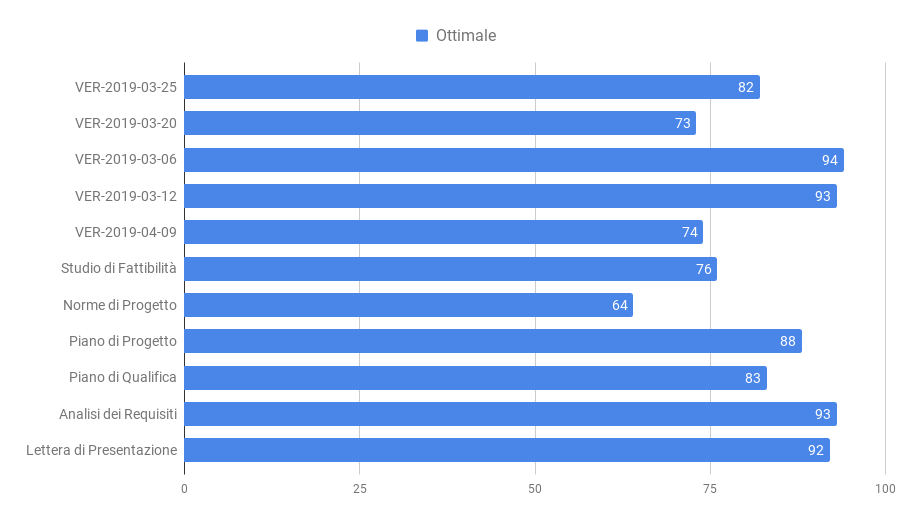
\includegraphics[scale=0.46]{immagini/GulpeaseG.png}
  \caption{Grafico valori indice Gulpease}
  \end{center}
\end{figure}


\subsubsection{M[PROD][S][0014]: Copertura del framework Octalysis}

\begin{table}[H]
\taburowcolors[2] 2{tableLineOne .. tableLineTwo}
\tabulinesep = 15pt
\everyrow{\tabucline[.4mm  white]{}}
\begin{tabu} to \textwidth { X[c,2] X[c,1] X[c,1] X[c,2] }
    \tableHeaderStyle
    Core Drive abbreviato & Quantità requisiti & Valore & Esito \\
    \textbf{Meaning} & 1 & 1 & Accettabile \\
    \textbf{Accomplishment} & 15 & 10 & Ottimo \\
    \textbf{Empowerment} & 1 & 1 & Accettabile  \\
    \textbf{Ownership} & 6 & 4 & Ottimo\\
    \textbf{Social Influence} & 5 & 3 &  Accettabile\\
    \textbf{Scarcity} & 0 & 0 & Ottimo\\
    \textbf{Unpredictability} & 2 & 1 & Ottimo\\
    \textbf{Avoidance} & 0 & 0 & Ottimo\\
\end{tabu}
\caption{Tabella resoconto copertura framework Octalysis}
\end{table}
\newpage
Il seguente grafico, ricavato tramite lo strumento online Octalysis-tool, riporta il codice di ogni requisito associato al relativo \citgl{Core Drive}. La dimensione di ogni area, identificata dal nome del Core Drive corrispondente, è proporzionale al valore raggiunto nella metrica sopra riportata.

\begin{figure}[h!]
\begin{center}
  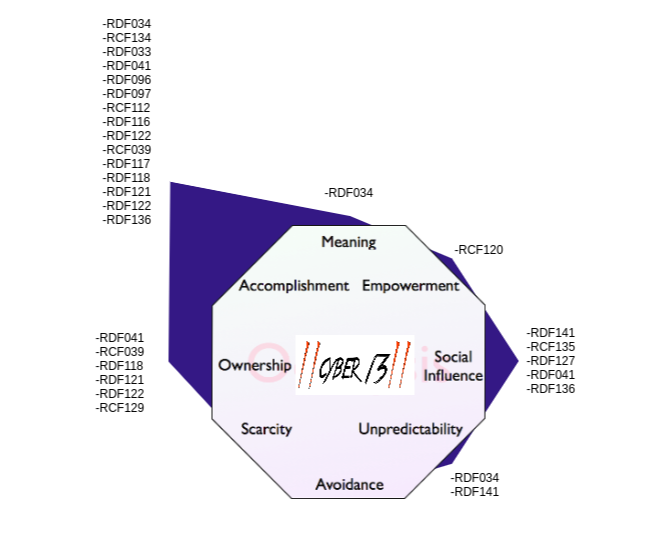
\includegraphics[scale=0.8]{immagini/Octalysys.png}
  \caption{Grafico copertura Core Drives Octalysys}
  \end{center}
\end{figure}



        
\end{document}
